\subthesischapter{Arquitectura del software}
En la aplicación se usó como arquitectura de software el MVC, un patrón de software comúnmente utilizado para implementar datos (Modelo), interfaces de usuario (Vista) y lógica de control (Controlador), que enfatiza una separación entre la lógica de negocios y su visualización. En la Figura~\ref{fig: software-architecture} se muestra el MVC correspondiente a la aplicación de juego serio.

\begin{figure}[ht]
    \centering
    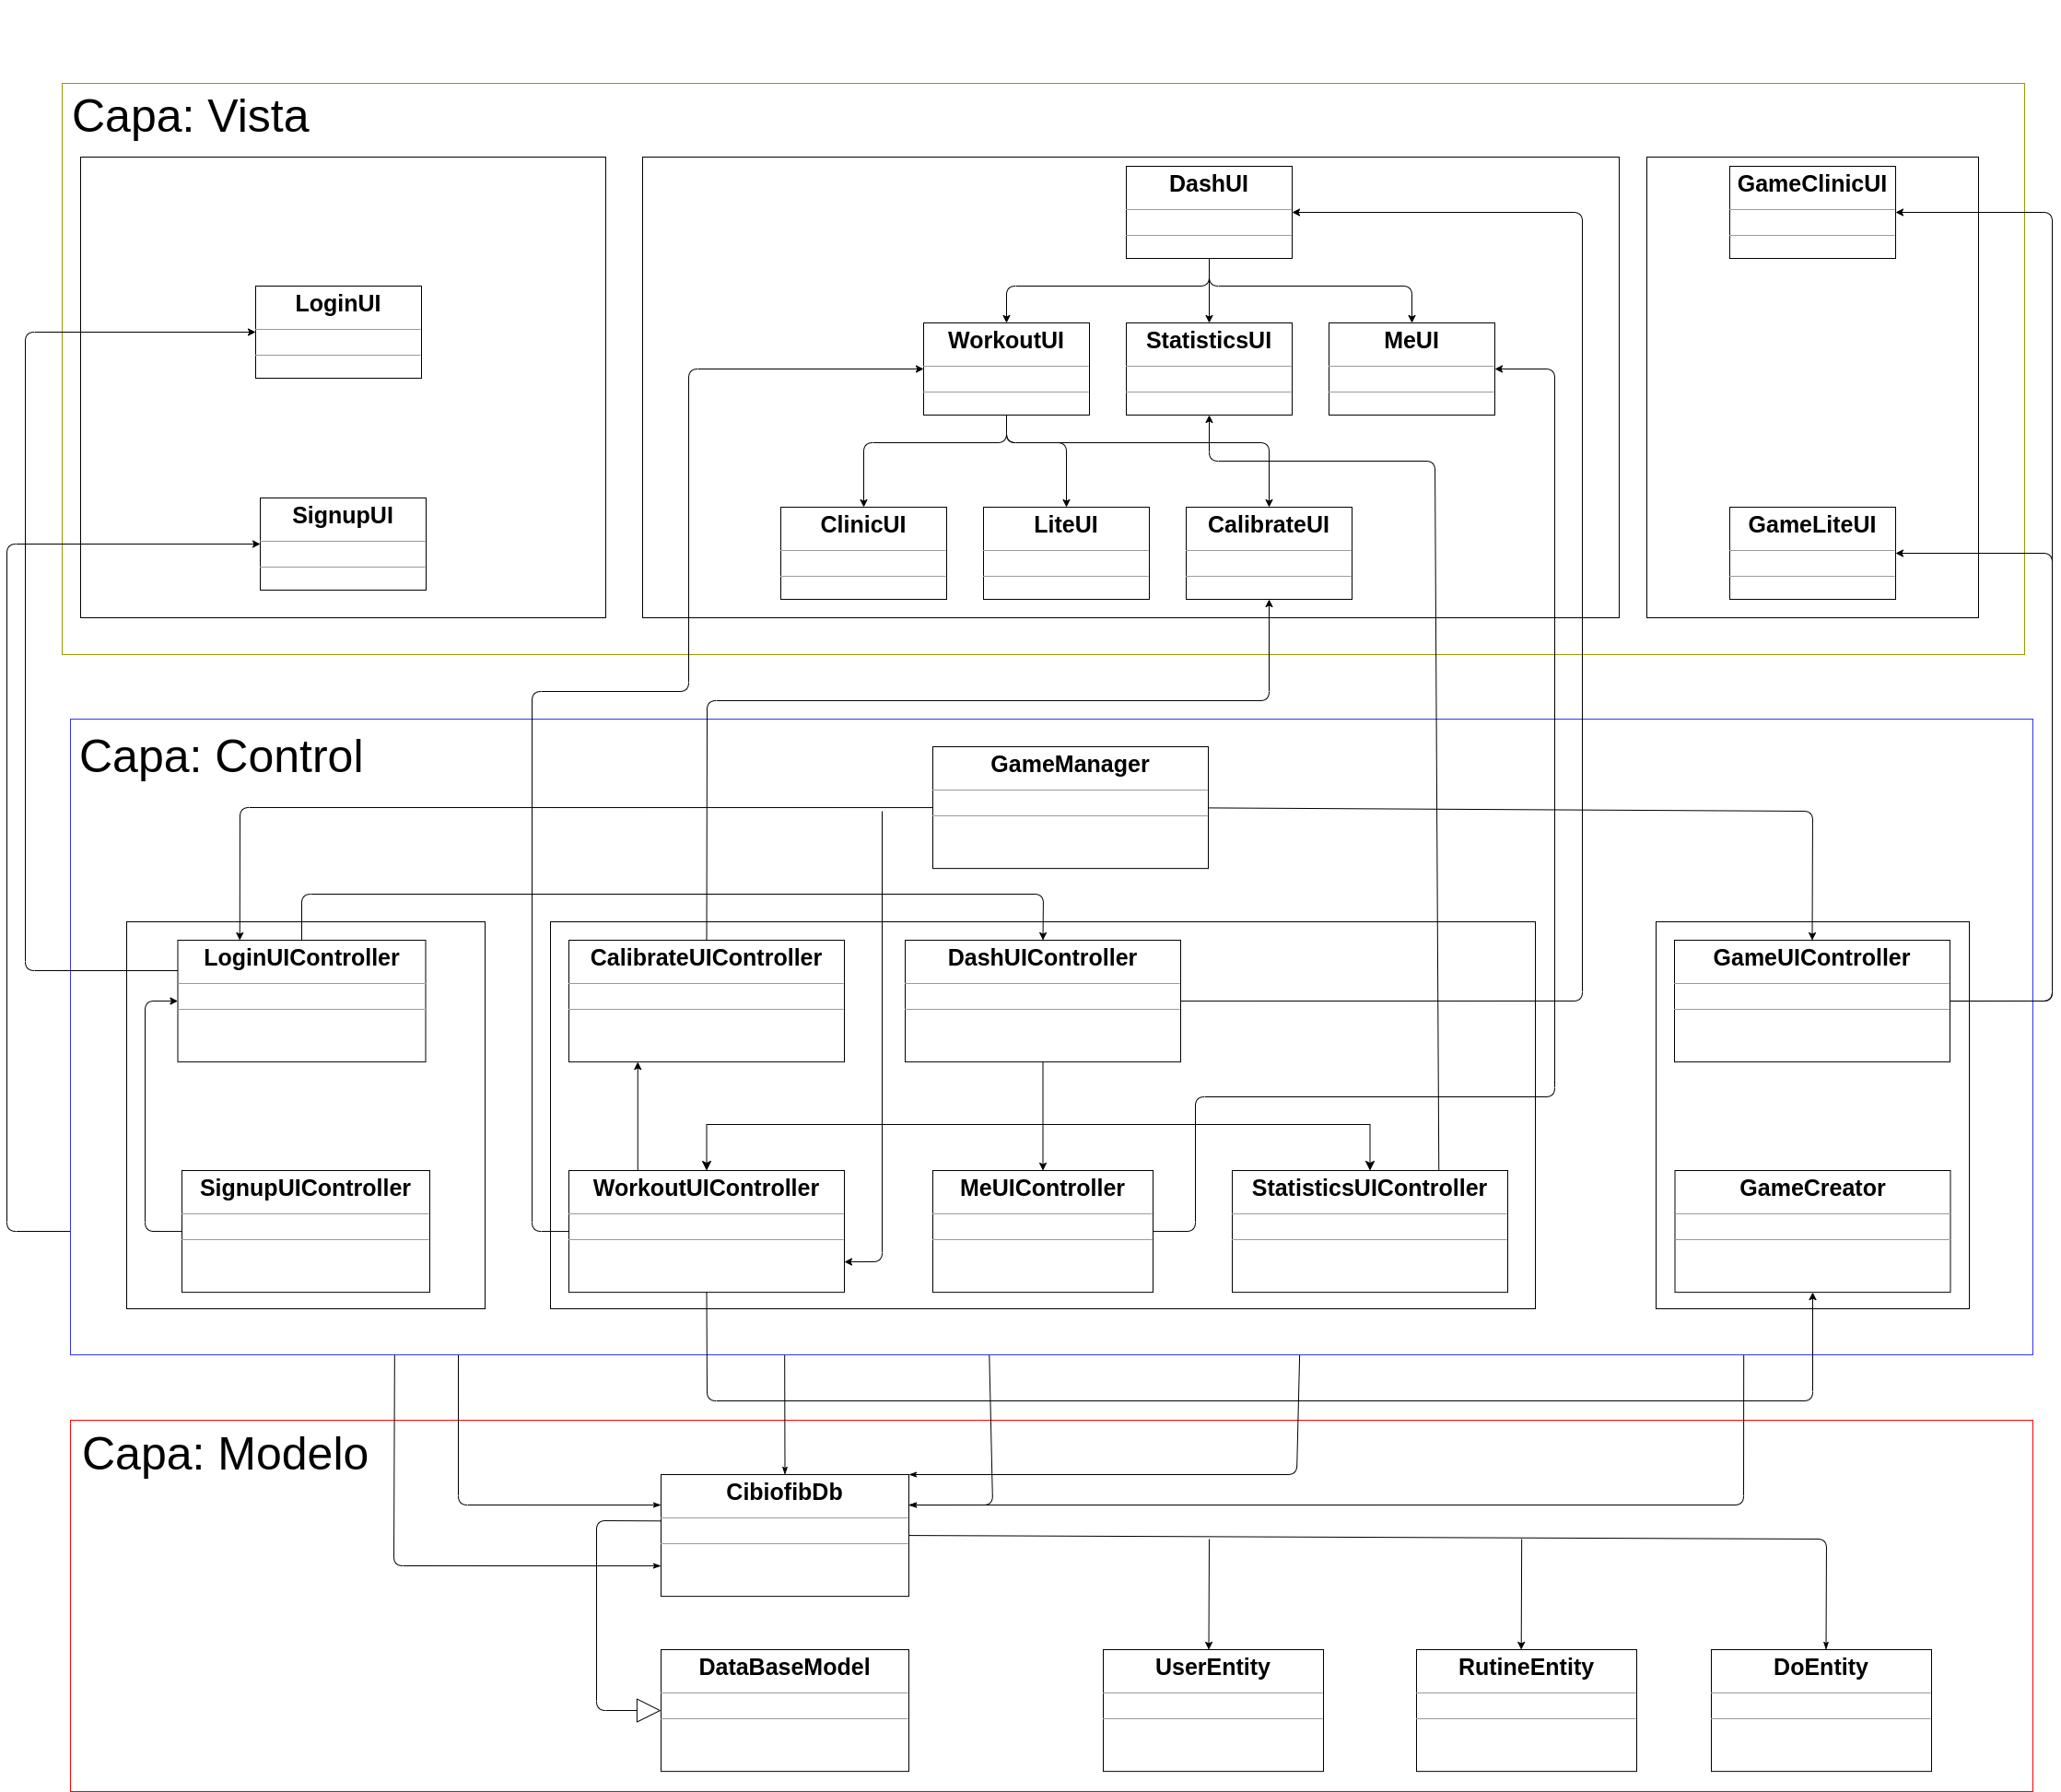
\includegraphics[scale=0.18]{images/software-architecture.png}
    \caption{Diagrama de clase de diseño}
    \label{fig: software-architecture}
\end{figure}

La arquitectura del MVC en el sistema se caracteriza por una clara separación de responsabilidades entre sus tres capas principales. El Modelo, representando la estructura interna de los datos, se vincula a la base de datos Cibiofib, asegurando la disponibilidad de la información en cada momento solicitado. Por otro lado, la capa de Vista proporciona un conjunto de vistas que definen las interfaces de la aplicación y son gestionadas por su respectivo controlador. Ejemplo: el acceso a la vista de configuraciones (MeUI) para el usuario es concedida a través del controlador (MeUIController). Dicho controlador carga los datos referentes al usuario y las rutinas configuradas que han sido almacenados en la base de datos y actualiza los componentes de dicha vista.






